\documentclass[12pt]{article}
\usepackage{amsmath}
\usepackage{amssymb}
\usepackage{geometry}
\usepackage{enumerate}
\usepackage{natbib}
\usepackage{float}%稳定图片位置
\usepackage{graphicx}%画图
\usepackage[english]{babel}
\usepackage{a4wide}
\usepackage{indentfirst}%缩进
\usepackage{enumerate}%加序号
\usepackage{multirow}%合并行
\title{\large UM-SJTU JOINT INSTITUTE\\Introduction to Computer Organization\\(VE370)\\\ \\\ \\\ \\\ \\\ \\\ \\\ \\\ \\\ \\\ \\\
Project 3\\\ \\\ Literature Research \\\ \\\ \\\ \\\ \\\ }
\author{Name: Pan Chongdan\\ID: 516370910121}
\date{Date: \today}

\begin{document}
\maketitle
\newpage
\section{Abstract}
Moore's Law, which was stated by Gordon Moore in 1965 states that the number of transistors on a integrated circuit plate of same size for double every 18 months. Accordingly, the cost of computer is also reduces by half every 18 moths so that we can get to computers so easily and quickly. Moore's Law has been proved to be valid for more than fifty years and it has stimulated the development of IT industry greatly. However, Moore's Law will fail in the end because the size of transistor can't be infinite small. My literature research will cover the factors leading to Moore's Law's failure and solution.
\section{Moore's Law's Limit}
\subsection{Size Problem}
At present, the scale of wire for chip is about 15nm, if it keep shrinking at current speed, the scale will be smaller than 5nm before 2020, which can only contains 10 atoms on the wire. Because of uncertainty of quantum, transistor won't be reliable.
\par In addition, if we shrink the size of the chip, the distance wires will become closer and closer, but when they're too close, quantum transition will probably happen so that electrons will jump from one wire to another so the circuit can't work any more.
\subsection{Material Problem}
Moore's first law define improved transistor drive current $$I_{dsat}=\beta (V_{gs}-V_t)^2/2$$ where $V_{gs}$ is the gate to source voltage, $V_t$ is the device threshold, and $β$ is the MOS transistor gain factor. The gain factor $/beta$ is dependent on both the process parameters and the device geometry, and is given by  
$$\beta=\mu\varepsilon/t_{ox}(W/L)$$ Where $\mu$ is the effective surface mobility of the carriers in the channel, $\varepsilon$ is the permittivity of the gate dielectric, $t_{ox}$ is the thickness of the gate dielectric, $W$ is the width of the channel and $L$ is the length of the channel. The gain factor $\beta$ thus consists of a process dependent factor $\mu\varepsilon/t_{ox}$, which contains all the process terms that account for such factors as doping density and gate oxide thickness. The process dependent factor is sometimes written as $\mu C_{ox}$ where $C_{ox}=\kappa\varepsilon_0 A/t_{ox}$, where $t_{ox}$ is limited by leakage and manufacturability. Thus the best options to increase the device performance are to increase $\kappa$ of the dielectric and improve the channel mobility.
\par Nowdays, $SiO_2$ are the best material used for transistors while we need to find high $\kappa$ dielectric to replace $Si O_2$. The new material must also achieve low electrical leakage and have negligible trap densities to meet gate leakage and reliability requirements. The require for new materials of low cost has been one of the most difficult problem to solve to keep Moore's Law.
\section{Solution}
\subsection{Cloud Computing}
Since we can't lower the cost of computers' on user's hands, we can just take the CPU out of the computer so that they won't worry about the size of the chip. With cloud computing technology, we can do the computation in the cloud and user's computer's just need to receive and send signals to the CPU in cloud.
\par In addition, if we build many CPU together in cloud, we can save the cost by building a super integrated CPU with other architecture which only designed for large scale calculation.
\subsection{More Moore's Law}
\begin{figure}[H]
\centering
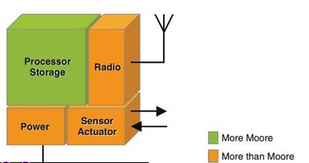
\includegraphics[scale=1.5]{P1.png}
\end{figure}
Currently, circuit are designed on one plane, according to "More Moore's Law" concept, they can be designed in three dimension. It can't improve the performance of circuit significantly, but it will reduce voltage leakage, which is called "Power-driven Technology Transition"
\subsection{More than Moore's Law}
"More than Moore's Law" focus on the variety of chip's function, which means opening minds and making more advance in other fields such sensor or power to improve product's performance instead of being stuck in figuring how to making smaller chips. For example, we can make more development on wireless communication and power transfer technology so our cell phone can work faster and longer. In addition, engineers can put more efforts on development virtual reality and artificial intelligence. 
\section{Conclusion}
In reality, there is always a limit for the size of transistor, but there is no limit for human's intelligence. So if we can decrease the cost of chips from other aspects like algorithm or architecture, there might be a chance that we can keep the Moore's Law 
\section{Reference}
\begin{enumerate}[-]
\item Robert R.Schaller. "Moore's Law: Past, Present and Future." IEEE Spectrum. June 1997.
\item Andrew B.Kahang. "Scaling: More than Moore's Law." IEEE Design $\&$ Test of Computers.
\item Young-Kai Chen. "More than Moore's law — Scaling with silicon photonics."2016 International Symposium on VLSI Technology, Systems and Application. 30 May 2016.
\item J.Prased "Challenges and opportunities for the universities to support future technology developments in the semiconductor industry: staying on the Moore's Law."  Proceedings of the 15th Biennial University/Government/ Industry Microelectronics Symposium. July 2003.
\end{enumerate}
\end{document}